\chapter{Literature Review}
\section{Introduction}

Hierdie projek vloei uit 'n voorstel van Mnr D.N.J.\ Els en vorm
ook deel van ...

\section{Audio Signal Fundamentals}

\subsection{Audio Frequency Range}

The audible frequency bandwidth of the human ear is widely considered to be \SI{20}{\hertz} to \SI{20}{\kilo\hertz}, \cite[p.~20]{Self:2009} and \cite[p.~42]{Slone:1999}. One would assume that when designing an audio amplifier you would take only this range into consideration, but this is untrue because of a phenomenon known as \textit{slew-induced distortion} or SID. When an amplifier cannot change its output voltage fast enough because of a rapidly changing or high frequency input signal, it tends to cause distortion at lower frequencies. For example, an inaudible \SI{30}{\kilo\hertz} signal could distort and interact with amplifier non-linearity, produce audible unwanted byproducts, \cite[p.~43]{Slone:1999}. We therefore should design our amplifier with a higher frequency bandwidth in mind.

\subsection{Distortion and Noise}

Linearity describes the extent to which the relationship between a circuit's input and output can be represented by a straight transfer characteristic \citep[p.~428]{Self:2009}. An ideal power amplifier's transfer function should be represented by a straight line in the form:

\begin{equation}
	v_{out} = A_v v_{in}
\end{equation}

Whereas a non-linear amplifier would behave approximately as:

\begin{equation}
	v_{\mathrm{out}}
	=
	a_1v_{\mathrm{in}}
	+
	a_2v_{\mathrm{in}}^2
	+
	a_3v_{\mathrm{in}}^3
	+
	\cdots
\end{equation}

The higher-order terms cause the gain to vary with instantaneous signal amplitude, thereby changing the waveform shape and generating harmonic or intermodulation distortion.

Distortion is unwanted change that an amplifier makes to the shape of an input signal. There are several sources of distortion in a power audio amplifier. The seven main causes of distortion are because of non-linearity in either the input stage, \textit{Voltage Amplification Stage} or VAS, output stage, non-linear input impedance loading of the VAS,  rail decoupling, induction of supply currents or NFB feed taken from the wrong place, \cite[p.~65-67]{Self:2009}.

\subsubsection{Input Stage Distortion}

Input stage distortion can be reduced by adding emitter degenration, \cite[p.~79-80]{Self:2009}, balancing the differential input pair, \cite[p.~80-82]{Self:2009} or increasing collector current whilst maintaining transconductance with emmiter degeneration resistors \cite[p.~86-87]{Self:2009}.

\subsubsection{VAS Distortion}

VAS distortion is caused by the curved qualities of the nonlinear \(V_{BE}\)--\(I_C\) transfer characteristic. The VAS can be linearised by increasing the local open loop gain to obtain greater local  \textit{Negative Feedback} or NFB, \cite{Self:2009}.

\subsubsection{Output Stage Distortion}

There are three main causes for distortion in the output stage, one of which is \textit{large-signal non-linearity} or LSN. LSN occurs when the amplifier's output devices must handle large voltage or current swings and their electrical behaviour is no longer constant. LSN can be reduced by increasing the number of output devices or choosing higher quality output devices \cite[p.~164-166]{Self:2009}.

The second is crossover distortion, which occurs a Class-B push-pull output stage during the transfer of control between the positive and negative output devices. This is eliminated with a Class-AB amplifier by applying a slight bias at your output stage.

The third is switching distortion which occurs when the output transistor that was conducting does not switch off quickly enough as the signal changes polarity. This can be fixed by using an output topology capable of reverse-biasing the output-transistor base-emitter junction during turn-off, particularly the EF Type II or using lower driver emitter or collector resistance so that stored charge is removed more quickly, \cite[p.~185]{Self:2009}.

\subsubsection{VAS-Loading Distortion}

VAS-Loading Distortion is caused by the non-linear loading of the output stage.

\subsubsection{Rail Decoupling Distortion}

\subsubsection{Induction Distortion}

\subsubsection{NFB take-off point Distortion}

\section{Audio Equalisation}

The main purpose of an audio equaliser circuit is to balance the different frequency bands present in an audio signal. For this project, it is required to design a equiliser centered around at least three frequency bands, the bass-, mid- and treble frequencies.

The graphic equiliser design from the Texas Instrument article, \cite{Carter:2001}, has been followed. The design uses simulated inductors and the article expands on equiliser qualities, such as the the bandwidth, gain and Q-values of the equiliser. 

A simulated inductor reverses the operation of a capacitor using an operational amplifier~\citep[p.~34]{Carter:2001}. Obtaining real inductors is expensive and difficult whereas a simulated inductor is inexpensive and has a smaller footprint.

Bandwidth is the range of frequencies affected by a one equiliser band and it is inversely correlated to its Q value. A higher Q value therefore displays a narrower, more pointy bandwidth as shown in Figure~\ref{fig:Q-Response} from \citep[p.~37]{Carter:2001}.

\begin{figure}[htbp]
	\centering
	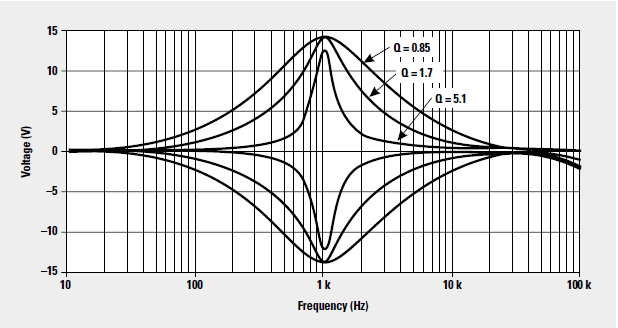
\includegraphics[width=1\textwidth]{Images/Literature Review/Bandwidth.png}
	\caption{Effect of Q on bandwidth for a graphic equalizer}
	\label{fig:Q-Response}
\end{figure}

The Q value is determined by the formula:

\begin{equation}
	Q = \dfrac{X_L}{R}
\end{equation}

Where the inductive reactance is determine by:

\begin{equation}
	X_L = 2\pi \times f_O \times L
\end{equation}

And the resonant frequency and simulated inductor is calculated with:

\begin{equation}
	f_O = \dfrac{1}{2\pi\sqrt{LC}}
\end{equation}

\begin{equation}
	L = (R5 - R4) \times R4 \times C1
\end{equation}

